\documentclass{standalone}
\usepackage{tikz}
\begin{document}
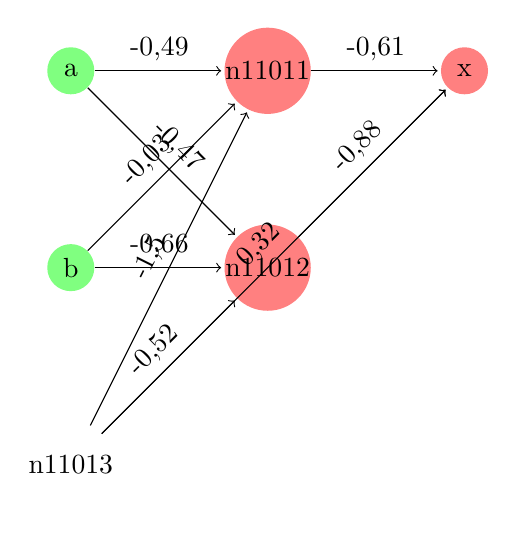
\begin{tikzpicture}[shorten >=1pt,->,draw=black!,node distance=2.5cm]
\tikzstyle{neuron}=[circle,fill=black!25,minimum size=17pt,inner sep=0pt]
\tikzstyle{constant}=[neuron, fill=white!50];
\tikzstyle{identity}=[neuron, fill=green!50];
\tikzstyle{sigmoid}=[neuron, fill=red!50];
\node [identity] (a) {a};
\node [identity,below of=a] (b) {b};
\node [constant,below of=b] (n11013) {n11013};
\node [sigmoid,right of=a] (n11011) {n11011};
\node [sigmoid,below of=n11011] (n11012) {n11012};
\node [sigmoid,right of=n11011] (x) {x};
\path[every node/.style={sloped,anchor=south,auto=false}]
(b) edge node {-0,03} (n11011)
(b) edge node {-0,66} (n11012)
(n11013) edge node {-0,52} (n11012)
(n11013) edge node {-1,5} (n11011)
(n11013) edge node {0,32} (x)
(n11011) edge node {-0,61} (x)
(n11012) edge node {-0,88} (x)
(a) edge node {-0,47} (n11012)
(a) edge node {-0,49} (n11011)
;\end{tikzpicture}
\end{document}